\documentclass[a4paper,12pt]{article}

\usepackage[spanish]{babel}
\usepackage[utf8]{inputenc}
\usepackage[T1]{fontenc}

%% Sets page size and margins
\usepackage[a4paper,margin=1in,marginparwidth=1in]{geometry}

%% Useful packages
\usepackage{amsmath}
\usepackage{breqn}
\usepackage{graphicx}
\usepackage[colorinlistoftodos]{todonotes}
\usepackage[colorlinks=true, allcolors=blue]{hyperref}
\usepackage{caption}
\usepackage{subcaption}
\usepackage{sectsty}
\usepackage{float}
\usepackage{titling} 
\usepackage{blindtext}
\usepackage[colorinlistoftodos]{todonotes}
\usepackage{xcolor}
\usepackage{textcomp}
\usepackage{hyperref}
\usepackage{fancyhdr}
\usepackage[style=ieee]{biblatex}
\usepackage{csquotes}
\usepackage{siunitx}
\usepackage{wrapfig}
\usepackage{amssymb}

\newcommand*{\field}[1]{\mathbb{#1}}%

\addbibresource{references.bib}
\definecolor{darkgreen}{rgb}{0.0, 0.4, 0.0}
\setlength{\headheight}{16pt}

\allowdisplaybreaks

\pagestyle{fancy}
\fancyhf{}
\rhead{Robótica}
\lhead{Manipulador \emph{{\textmu}Arm}}
\cfoot{\thepage}

%%%%%%%% DOCUMENT %%%%%%%%
\begin{document}

%%%% Title Page
\begin{titlepage}

    \newcommand{\HRule}{\rule{\linewidth}{0.5mm}}
    \center

    % University
    \textsc{\LARGE Universidad Politécnica de Madrid}\\[1cm]

    % Document info
    \textsc{\Large Robótica}\\[0.2cm]
    \textsc{\large \textit{MANIPULADORES}}\\[1cm]
    \HRule \\[0.8cm]
    { \huge \bfseries Estudio del manipulador \textit{{\textmu}Arm}}\\[0.7cm]
    \HRule \\[2cm]
    \large
    \emph{Autores:}\\
    Javier Alonso Silva - \href{mailto:javier.asilva@alumnos.upm.es}{javier.asilva@alumnos.upm.es}

    Roberto Álvarez Garrido - \href{mailto:roberto.alvarezg@alumnos.upm.es}{roberto.alvarezg@alumnos.upm.es}

    José Alejandro Moya Blanco - \href{mailto:alejandro.moya.blanco@alumnos.upm.es}{alejandro.moya.blanco@alumnos.upm.es}\\[1.5cm]
    {\large Última modificación: \today}\\[2cm]
    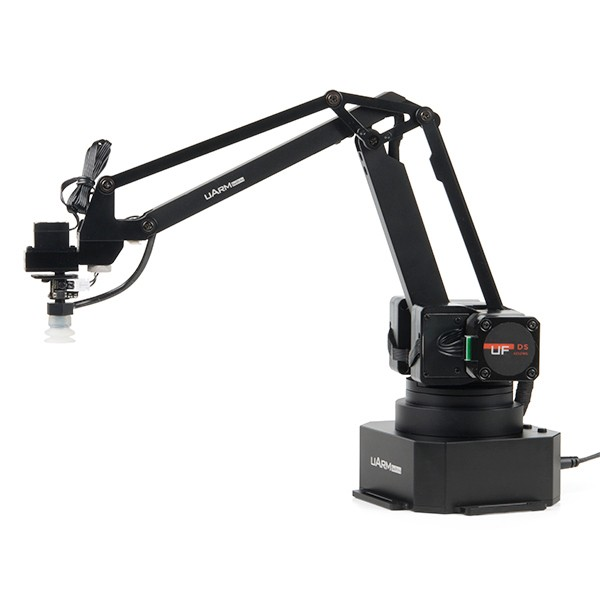
\includegraphics[width=0.5\textwidth]{images/uarm.jpg}\\[1cm]
\end{titlepage}

%%%% SECTIONS
\section*{Conocimientos previos}
\label{sec:previous_knowledge}

Antes de ponernos a hablar sobre los resultados obtenidos en la práctica,
antes vamos a hablar sobre algunas características básicas del brazo robótico e
introducirlo brevemente.
El manipulador robótico \emph{{\textmu}Arm} es un dispositivo creado por la empresa
\href{https://www.ufactory.cc/#/}{UFACTORY} el cual cuenta con cuatro grados de libertad.
De dichos grados de libertad, tres son usados para mover el brazo robótico hasta ciertas
posiciones y, el último, para mantener el extremo del mismo paralelo al suelo.

\begin{wrapfigure}{R}{.4\textwidth}
    \begin{center}
        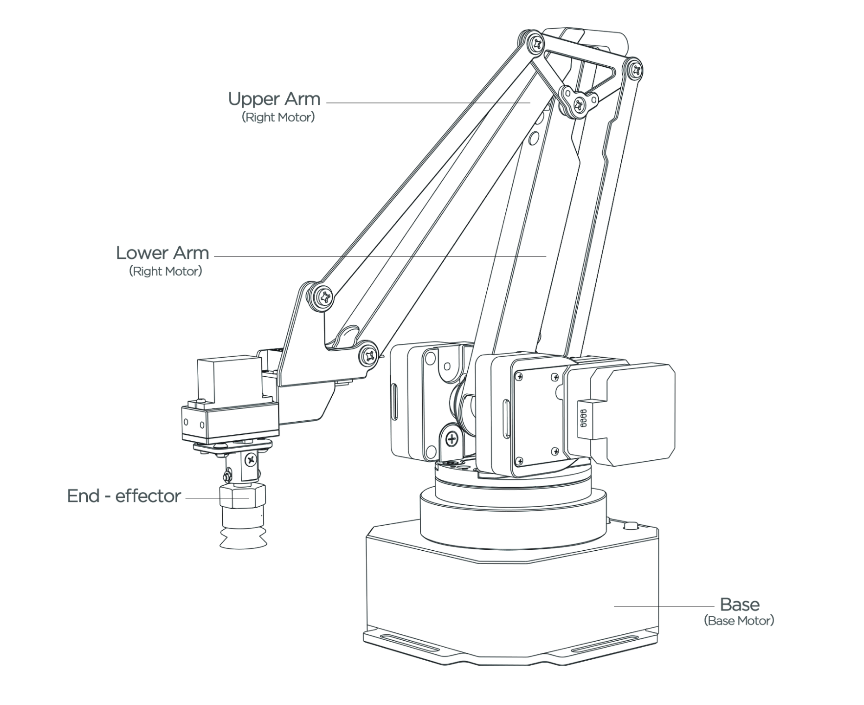
\includegraphics[width=.4\textwidth]{images/motors.png}
        \caption{zonas de actuación de los motores en el brazo \cite{noauthor_uarm_2019-1}}
        \label{fig:motors}
    \end{center}
\end{wrapfigure}

El manipulador es controlado mediante cuatro motores:

% \begin{itemize}
El \textbf{motor de la base} el cual permite la rotación del manipulador.

En el brazo, el \textbf{motor que está a la derecha} (ver la figura \ref{fig:motors}),
coordina el movimiento de la parte inferior del brazo (\textit{Lower Arm} en la figura)
con la parte superior del mismo (\textit{Upper Arm} en la figura).

En esta parte del manipulador, el movimiento es como el de un flexo: la parte superior
del flexo está supeditada a la parte inferior, de manera que se mantiene de forma
constante la altura a la que está el extremo final del mismo.

El otro motor, localizado a la \textbf{izquierda del brazo}, se encarga de mantener la
orientación del extremo del manipulador. De esta manera, dicho extremo
permanecerá paralelo al suelo. Teniendo en cuenta esto, podríamos decir
que el robot en verdad solo tiene tres grados de libertad en tanto a que no se
controla directamente el movimiento del último grado, ya que al final se mueve
para permanecer paralelo al suelo.

El \textbf{motor localizado en el extremo}, con el cual se puede actuar sobre el
elemento que esté colocado allí. Por ejemplo, cuando se coloca una ventosa
permite rotarla o, cuando se coloca la pinza, el movimiento del motor permite
abrirla o cerrarla.

Para este estudio, este último motor se descartará, ya que no afecta a las
posiciones accesibles por el robot.
% \end{itemize}

\begin{table}[ht]
    \begin{minipage}{.49\linewidth}
        \centering
        \begin{tabular}{||c | c||}
            \hline
            \textit{Motor} & \textit{Rango de trabajo} \\ [0.5ex]
            \hline\hline
            Base           & $\ang{0} \sim \ang{180}$  \\
            \hline
            Derecho        & $\ang{0} \sim \ang{130}$  \\
            \hline
            Izquierdo      & $\ang{0} \sim \ang{106}$  \\
            \hline
            Extremo        & $\ang{0} \sim \ang{180}$  \\ [1ex]
            \hline
        \end{tabular}
        \caption{ángulo de giro de los motores \cite{noauthor_uarm-swift-specifications-171012.pdf_2019}}
        \label{tab:motors}
    \end{minipage}
    \hfill
    \begin{minipage}{.49\linewidth}
        \begin{figure}[H]
            \centering
            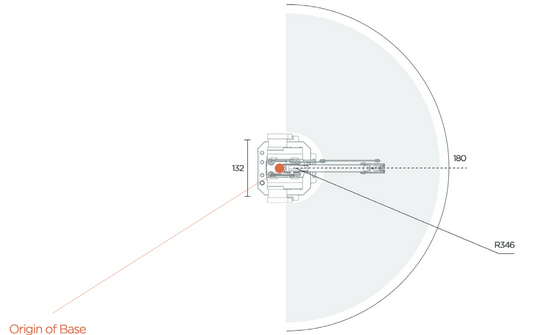
\includegraphics[width=\linewidth]{images/range.png}
            \caption{rango del manipulador \emph{{\textmu}Arm} \cite{noauthor_uarm_2019}}
            \label{fig:range}
        \end{figure}
    \end{minipage}
\end{table}

\newpage
Toda la información relativa al desarrollo del proyecto puede ser encontrada en
\href{https://github.com/UPM-Robotics/uarm}{GitHub - UPM Robotics} \cite{noauthor_upm-robotics/uarm_2019}. Allí están detallados
los distintos hitos a conseguir así como más información sobre el robot.

Además, se encuentra disponible la siguiente bibliografía:
\begin{itemize}
    \item \href{https://github.com/UPM-Robotics/uarm/blob/master/docs/robot-information/uArm%20pro%20User%20Manual%20v1.1.0.pdf}{Manual de usuario}
    \item \href{https://github.com/UPM-Robotics/uarm/blob/master/docs/robot-information/uArm-Swift-Specifications-171012.pdf}{Especificaciones}
    \item \href{https://github.com/UPM-Robotics/uarm/blob/master/docs/robot-information/uArm%20Swift%20Pro_Developer%20Guide%20v1.0.6.pdf}{Guía del desarrollador}
    \item \href{https://github.com/UPM-Robotics/uarm/blob/master/docs/robot-information/uArm_Swift_Pro_3D_20180620.STEP}{Modelo en 3D}
    \item \href{https://www.ufactory.cc/#/en/}{Web de UFACTORY}
    \item \href{https://www.ufactory.cc/#/en/support/technology}{Soporte de UFACTORY}
\end{itemize}

\newpage
\section{Configuración geométrica}
\label{sec:dk}

En esta sección vamos a describir la configuración geométrica del brazo robótico. La
configuración que obtuvimos fue la siguiente:
\begin{figure}[H]
    \begin{minipage}{.4\linewidth}
        \centering
        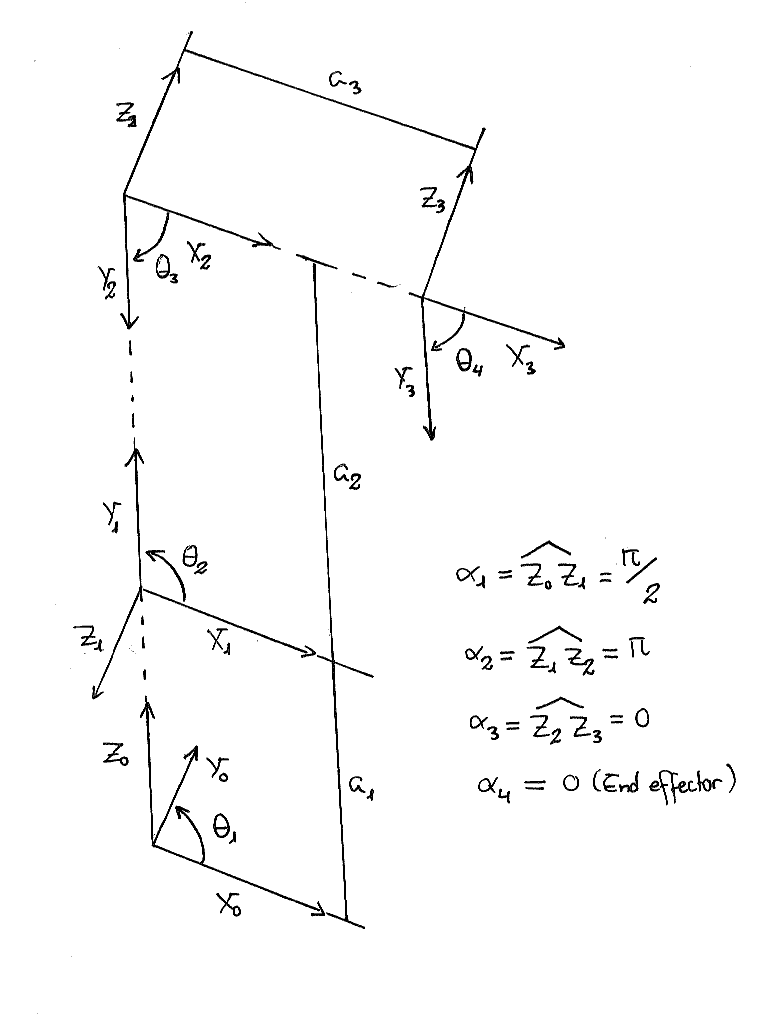
\includegraphics[width=\linewidth]{images/geometric_configuration_2.png}
        \caption{configuración geométrica del robot}
        \label{fig:robot_config}
    \end{minipage}\hfill
    \begin{minipage}{.48\linewidth}
        \centering
        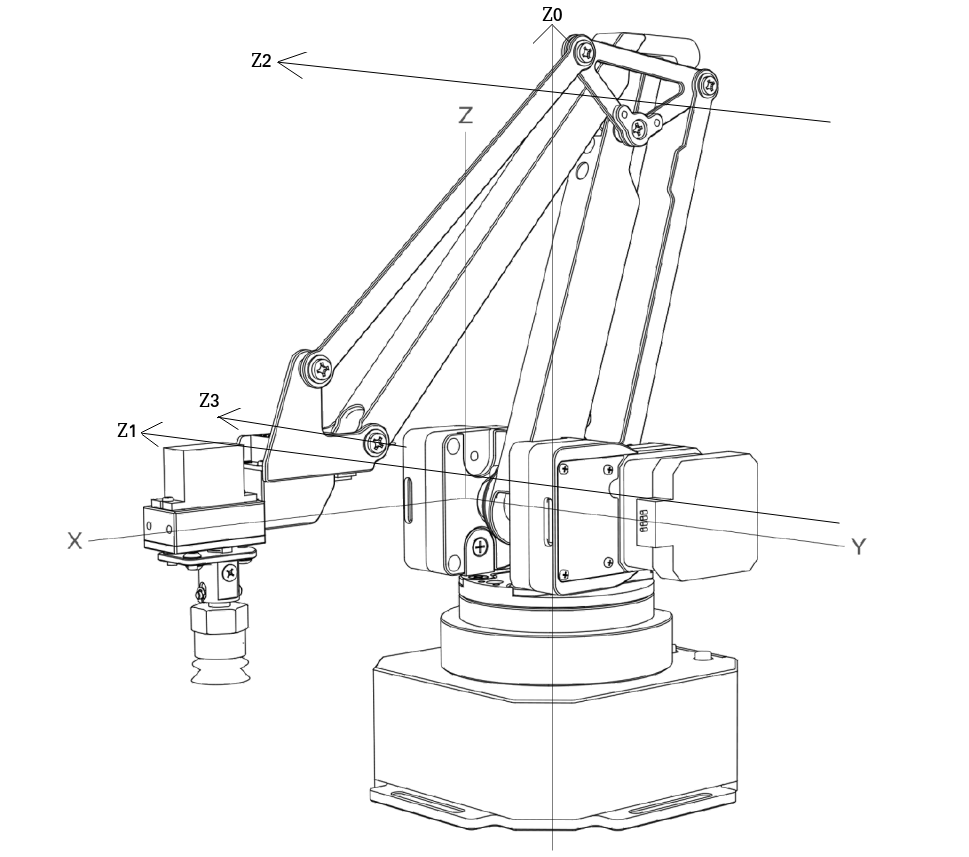
\includegraphics[width=\linewidth]{images/axis.png}
        \caption{los grados de libertar del brazo, representados por los diferentes $Z_i$}
        \label{fig:axis}
    \end{minipage}
\end{figure}

Usando los datos que están presentes en la documentación al desarrollador \cite{noauthor_uarm_2019-1},
pudimos obtener los siguientes datos para los $a_i$ (distancia entre ejes) del manipulador; además,
descubrimos que hay una pequeña desviación $d_i$ entre las articulaciones $\{1, 2\}$:

\begin{table}[ht]
    \begin{minipage}{.49\linewidth}
        \begin{figure}[H]
            \centering
            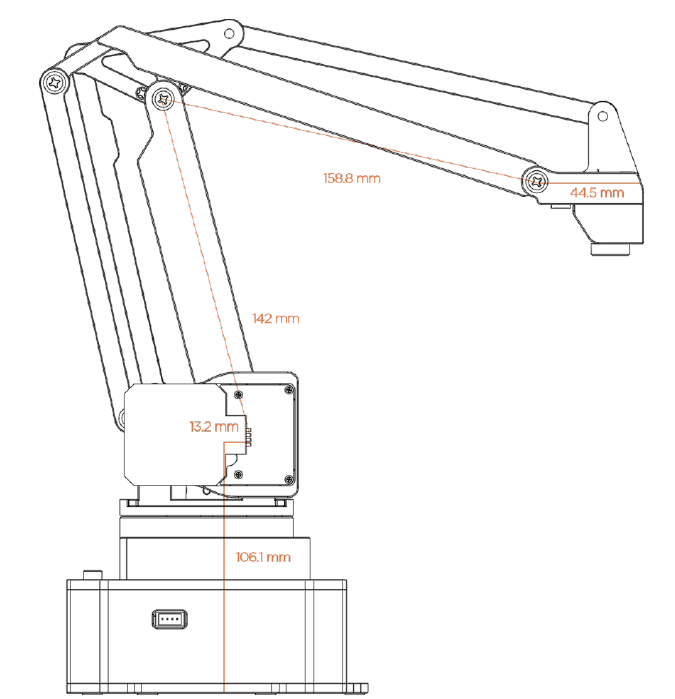
\includegraphics[width=\linewidth]{images/sizes.png}
            \caption{longitudes del brazo robótico \cite{noauthor_uarm_2019-1}}
            \label{fig:sizes}
        \end{figure}
    \end{minipage}
    \hfill
    \begin{minipage}{.49\linewidth}
        \centering
        \begin{tabular}{|| c | c c ||}
            \hline
            $i$ & $a_i~(mm.)$ & $d_i~(mm.)$ \\ [0.5ex]
            \hline\hline
            $1$ & $106.1$     & $13.2$      \\
            \hline
            $2$ & $142$       & $0$         \\
            \hline
            $3$ & $158.8$     & $0$         \\
            \hline
            $4$ & $44.5$      & $0$         \\ [1ex]
            \hline
        \end{tabular}
        \caption{longitudes y desviaciones del manipulador}
    \end{minipage}
\end{table}

De esta manera, con los datos obtenidos, generamos una primera matriz de \textit{Denavit-Hartenberg}:

\begin{table}[H]
    \parbox{.45\linewidth}{
        \centering
        \begin{tabular}{ c | c c c c }
            $i$ & $\theta_i$ & $d_i~(mm.)$ & $a_i~(mm.)$ & $\alpha_i$      \\ [0.5ex]
            \hline
            $1$ & $\theta_1$ & $13.2$      & $106.1$     & $\frac{\pi}{2}$ \\
            $2$ & $\theta_2$ & $0$         & $142$       & $\pi$           \\
            $3$ & $\theta_3$ & $0$         & $158.8$     & $0$             \\
            $4$ & $\theta_4$ & $0$         & $44.5$      & $0$             \\ [1ex]
        \end{tabular}
        \caption{primera tabla de \textit{Denavit–Hartenberg}}
    }
    \hfill
    \parbox{.45\linewidth}{
        \centering
        \begin{tabular}{ c | c c c c }
            $i$ & $\theta_i$ & $d_i~(mm.)$ & $a_i~(mm.)$ & $\alpha_i$      \\ [0.5ex]
            \hline
            $1$ & $\theta_1$ & $d_1$       & $a_1$       & $\frac{\pi}{2}$ \\
            $2$ & $\theta_2$ & $0$         & $a_2$       & $\pi$           \\
            $3$ & $\theta_3$ & $0$         & $a_3$       & $0$             \\
            $4$ & $\theta_4$ & $0$         & $a_4$       & $0$             \\ [1ex]
        \end{tabular}
        \caption{primera tabla de \textit{Denavit–Hartenberg} parametrizada}
    }
\end{table}

La cuestión es que, al hacer los distintos modelos, descubrimos que debido a la orientación del brazo
robótico, la $d_i$ está en la posición del equivalente $a_i$, en particular $d_1$ y $a_1$.
Esto es debido a que, como se puede ver en la figura \ref{fig:axis} junto con las figuras \ref{fig:robot_config}
y \ref{fig:sizes}, el plano sobre el que está $d_i$ es el $XZ$, lo cual nos obliga a cambiar las posiciones
en las que existen a la vez un $a_i$ y un $d_i$, siempre y cuando ambos sean constantes, que en este caso lo son.
De esta forma, la tabla de \textit{Denavit-Hartenberg} quedaría:

\begin{table}[H]
    \parbox{.45\linewidth}{
        \centering
        \begin{tabular}{ c | c c c c }
            $i$ & $\theta_i$ & $d_i~(mm.)$ & $a_i~(mm.)$ & $\alpha_i$      \\ [0.5ex]
            \hline
            $1$ & $\theta_1$ & $106.1$     & $13.2$      & $\frac{\pi}{2}$ \\
            $2$ & $\theta_2$ & $0$         & $142$       & $\pi$           \\
            $3$ & $\theta_3$ & $0$         & $158.8$     & $0$             \\
            $4$ & $\theta_4$ & $0$         & $44.5$      & $0$             \\ [1ex]
        \end{tabular}
        \caption{segunda tabla de \textit{Denavit–Hartenberg}}
    }
    \hfill
    \parbox{.45\linewidth}{
        \centering
        \begin{tabular}{ c | c c c c }
            $i$ & $\theta_i$ & $d_i~(mm.)$ & $a_i~(mm.)$ & $\alpha_i$      \\ [0.5ex]
            \hline
            $1$ & $\theta_1$ & $a_1$       & $d_1$       & $\frac{\pi}{2}$ \\
            $2$ & $\theta_2$ & $0$         & $a_2$       & $\pi$           \\
            $3$ & $\theta_3$ & $0$         & $a_3$       & $0$             \\
            $4$ & $\theta_4$ & $0$         & $a_4$       & $0$             \\ [1ex]
        \end{tabular}
        \caption{segunda tabla de \textit{Denavit–Hartenberg} parametrizada}
    }
\end{table}

Finalmente, el \textit{end-effector} (véase la figura \ref{fig:motors}) siempre está perpendicular
al plano del suelo, es decir, $\phi_e = \pi$. Por eso mismo, el parámetro $i = 4$ en verdad
está supeditado siempre al movimiento que se realice según los ángulos $\theta_2$ y $\theta_3$, así
que no es necesario contemplarlo en la tabla de \textit{Denavit-Hartenberg}:

\begin{table}[H]
    \parbox{.45\linewidth}{
        \centering
        \begin{tabular}{ c | c c c c }
            $i$ & $\theta_i$ & $d_i~(mm.)$ & $a_i~(mm.)$ & $\alpha_i$      \\ [0.5ex]
            \hline
            $1$ & $\theta_1$ & $106.1$     & $13.2$      & $\frac{\pi}{2}$ \\
            $2$ & $\theta_2$ & $0$         & $142$       & $\pi$           \\
            $3$ & $\theta_3$ & $0$         & $158.8$     & $0$             \\ [1ex]
        \end{tabular}
        \caption{tabla de \textit{Denavit–Hartenberg}}
    }
    \hfill
    \parbox{.45\linewidth}{
        \centering
        \begin{tabular}{ c | c c c c }
            $i$ & $\theta_i$ & $d_i~(mm.)$ & $a_i~(mm.)$ & $\alpha_i$      \\ [0.5ex]
            \hline
            $1$ & $\theta_1$ & $a_1$       & $d_1$       & $\frac{\pi}{2}$ \\
            $2$ & $\theta_2$ & $0$         & $a_2$       & $\pi$           \\
            $3$ & $\theta_3$ & $0$         & $a_3$       & $0$             \\ [1ex]
        \end{tabular}
        \caption{tabla de \textit{Denavit–Hartenberg} parametrizada}
    }
\end{table}
\newpage
\section{Cinemática directa}
A continuación, con los valores obtenidos en el apartado anterior, vamos a obtener las
distintas matrices de transformación de referenciales de manipuladores. Para ello, partimos de la
siguiente matriz:

\[
    A_{i-1}^i =
    \begin{pmatrix}
        \cos\theta_i & -\cos\alpha_i\sin\theta_i & \sin\alpha_i\sin\theta_i  & a_i\cos\theta_i \\
        \sin\theta_i & \cos\alpha_i\cos\theta_i  & -\sin\alpha_i\cos\theta_i & a_i\sin\theta_i \\
        0            & \sin\alpha_i              & \cos\alpha_i              & d_i             \\
        0            & 0                         & 0                         & 1
    \end{pmatrix}
\]

Aplicando los distintos pasos, obtenemos:

\begin{align*}
    A_0^1 & =
    \begin{pmatrix}
        \cos{\left(\theta_{1} \right)} & 0 & \sin{\left(\theta_{1} \right)}   & d_{1} \cos{\left(\theta_{1} \right)} \\
        \sin{\left(\theta_{1} \right)} & 0 & - \cos{\left(\theta_{1} \right)} & d_{1} \sin{\left(\theta_{1} \right)} \\
        0                              & 1 & 0                                & a_{1}                                \\
        0                              & 0 & 0                                & 1                                    \\
    \end{pmatrix} \\
    A_1^2 & =
    \begin{pmatrix}
        \cos{\left(\theta_{2} \right)} & \sin{\left(\theta_{2} \right)}   & 0  & a_{2} \cos{\left(\theta_{2} \right)} \\
        \sin{\left(\theta_{2} \right)} & - \cos{\left(\theta_{2} \right)} & 0  & a_{2} \sin{\left(\theta_{2} \right)} \\
        0                              & 0                                & -1 & 0                                    \\
        0                              & 0                                & 0  & 1                                    \\
    \end{pmatrix} \\
    A_2^3 & =
    \begin{pmatrix}
        \cos{\left(\theta_{3} \right)} & - \sin{\left(\theta_{3} \right)} & 0 & a_{3} \cos{\left(\theta_{3} \right)} \\
        \sin{\left(\theta_{3} \right)} & \cos{\left(\theta_{3} \right)}   & 0 & a_{3} \sin{\left(\theta_{3} \right)} \\
        0                              & 0                                & 1 & 0                                    \\
        0                              & 0                                & 0 & 1                                    \\
    \end{pmatrix}
\end{align*}

Con todas las matrices ya obtenidas, podemos calcular la matriz de
transformación directa del manipulador (son 4 columnas, sin embargo no cabe la matriz al completo y por eso la última columna está debajo):

{\footnotesize\begin{align*}
    A_0^2 & =
    \begin{pmatrix}
        \cos{\left(\theta_{1} \right)} \cos{\left(\theta_{2} \right)} & \sin{\left(\theta_{2} \right)} \cos{\left(\theta_{1} \right)} & - \sin{\left(\theta_{1} \right)} & \left(a_{2} \cos{\left(\theta_{2} \right)} + d_{1}\right) \cos{\left(\theta_{1} \right)} \\
        \sin{\left(\theta_{1} \right)} \cos{\left(\theta_{2} \right)} & \sin{\left(\theta_{1} \right)} \sin{\left(\theta_{2} \right)} & \cos{\left(\theta_{1} \right)}   & \left(a_{2} \cos{\left(\theta_{2} \right)} + d_{1}\right) \sin{\left(\theta_{1} \right)} \\
        \sin{\left(\theta_{2} \right)}                                & - \cos{\left(\theta_{2} \right)}                              & 0                                & a_{1} + a_{2} \sin{\left(\theta_{2} \right)}                                             \\
        0                                                             & 0                                                             & 0                                & 1                                                                                        \\
    \end{pmatrix} \\
    A_0^3 & =
    \begin{pmatrix}
        \cos{\left(\theta_{1} \right)} \cos{\left(\theta_{2} - \theta_{3} \right)} & \sin{\left(\theta_{2} - \theta_{3} \right)} \cos{\left(\theta_{1} \right)}                                                                          & - \sin{\left(\theta_{1} \right)} \\
        \sin{\left(\theta_{1} \right)} \cos{\left(\theta_{2} - \theta_{3} \right)} & \sin{\left(\theta_{1} \right)} \sin{\left(\theta_{2} - \theta_{3} \right)}                                                                          & \cos{\left(\theta_{1} \right)}   \\
        \sin{\left(\theta_{2} - \theta_{3} \right)}                                & - \cos{\left(\theta_{2} - \theta_{3} \right)}                                                                                                       & 0                                \\
        0                                                                          & 0                                                                                                                                                   & 0                                \\
                                                                                   & \qquad \left(a_{2} \cos{\left(\theta_{2} \right)} + a_{3} \cos{\left(\theta_{2} - \theta_{3} \right)} + d_{1}\right) \cos{\left(\theta_{1} \right)}                                    \\
                                                                                   & \qquad \left(a_{2} \cos{\left(\theta_{2} \right)} + a_{3} \cos{\left(\theta_{2} - \theta_{3} \right)} + d_{1}\right) \sin{\left(\theta_{1} \right)}                                    \\
                                                                                   & \qquad a_{1} + a_{2} \sin{\left(\theta_{2} \right)} + a_{3} \sin{\left(\theta_{2} - \theta_{3} \right)}                                                                                \\
                                                                                   & \qquad 1
    \end{pmatrix}
\end{align*}}

\newpage
Las matrices están parametrizadas. Numéricamente, la matriz de transformación directa $A_0^3$ quedaría:

{\footnotesize\begin{align*}
    A_0^3 & =
    \begin{pmatrix}
        \cos{\left(\theta_{1} \right)} \cos{\left(\theta_{2} - \theta_{3} \right)} & \sin{\left(\theta_{2} - \theta_{3} \right)} \cos{\left(\theta_{1} \right)}                                                                         & - \sin{\left(\theta_{1} \right)} \\
        \sin{\left(\theta_{1} \right)} \cos{\left(\theta_{2} - \theta_{3} \right)} & \sin{\left(\theta_{1} \right)} \sin{\left(\theta_{2} - \theta_{3} \right)}                                                                         & \cos{\left(\theta_{1} \right)}   \\
        \sin{\left(\theta_{2} - \theta_{3} \right)}                                & - \cos{\left(\theta_{2} - \theta_{3} \right)}                                                                                                      & 0                                \\
        0                                                                          & 0                                                                                                                                                  & 0                                \\
                                                                                   & \qquad \left(142.0 \cos{\left(\theta_{2} \right)} + 158.9 \cos{\left(\theta_{2} - \theta_{3} \right)} + 13.2\right) \cos{\left(\theta_{1} \right)}                                    \\
                                                                                   & \qquad \left(142.0 \cos{\left(\theta_{2} \right)} + 158.9 \cos{\left(\theta_{2} - \theta_{3} \right)} + 13.2\right) \sin{\left(\theta_{1} \right)}                                    \\
                                                                                   & \qquad 142.0 \sin{\left(\theta_{2} \right)} + 158.9 \sin{\left(\theta_{2} - \theta_{3} \right)} + 106.1                                                                               \\
                                                                                   & \qquad 1                                                                                                                                                                              \\
    \end{pmatrix}
\end{align*}}

Finalmente, hay que añadir una traslación\footnote{$T_X$ es la traslación en $X$, mientras que $T_Z$ es la traslación en $Z$} en el eje $Z$ (debido a la posición del \textit{end-effector})
y en el eje $X$, ya que después de la articulación $\theta_3$ hay una extensión de $44,5~mm.$ (ver figura \ref{fig:sizes}),
para obtener así la posición final del robot $(X_e ~ Y_e ~ Z_e)$:

{\footnotesize\begin{align}
    A_0^3 & =
    \begin{pmatrix}
        \cos{\left(\theta_{1} \right)} \cos{\left(\theta_{2} - \theta_{3} \right)} & \sin{\left(\theta_{2} - \theta_{3} \right)} \cos{\left(\theta_{1} \right)}                                                                                & - \sin{\left(\theta_{1} \right)} \\
        \sin{\left(\theta_{1} \right)} \cos{\left(\theta_{2} - \theta_{3} \right)} & \sin{\left(\theta_{1} \right)} \sin{\left(\theta_{2} - \theta_{3} \right)}                                                                                & \cos{\left(\theta_{1} \right)}   \\
        \sin{\left(\theta_{2} - \theta_{3} \right)}                                & - \cos{\left(\theta_{2} - \theta_{3} \right)}                                                                                                             & 0                                \\
        0                                                                          & 0                                                                                                                                                         & 0                                \\
                                                                                   & \qquad \left(a_{2} \cos{\left(\theta_{2} \right)} + a_{3} \cos{\left(\theta_{2} - \theta_{3} \right)} + d_{1}\right) \cos{\left(\theta_{1} \right)} + T_X                                    \\
                                                                                   & \qquad \left(a_{2} \cos{\left(\theta_{2} \right)} + a_{3} \cos{\left(\theta_{2} - \theta_{3} \right)} + d_{1}\right) \sin{\left(\theta_{1} \right)}                                          \\
                                                                                   & \qquad a_{1} + a_{2} \sin{\left(\theta_{2} \right)} + a_{3} \sin{\left(\theta_{2} - \theta_{3} \right)} - T_{Z}                                                                              \\
                                                                                   & \qquad 1
    \end{pmatrix} \label{eq:A03_param} \\
    A_0^3 & =
    \begin{pmatrix}
        \cos{\left(\theta_{1} \right)} \cos{\left(\theta_{2} - \theta_{3} \right)} & \sin{\left(\theta_{2} - \theta_{3} \right)} \cos{\left(\theta_{1} \right)}                                                                         & - \sin{\left(\theta_{1} \right)} \\
        \sin{\left(\theta_{1} \right)} \cos{\left(\theta_{2} - \theta_{3} \right)} & \sin{\left(\theta_{1} \right)} \sin{\left(\theta_{2} - \theta_{3} \right)}                                                                         & \cos{\left(\theta_{1} \right)}   \\
        \sin{\left(\theta_{2} - \theta_{3} \right)}                                & - \cos{\left(\theta_{2} - \theta_{3} \right)}                                                                                                      & 0                                \\
        0                                                                          & 0                                                                                                                                                  & 0                                \\
                                                                                   & \left(142.0 \cos{\left(\theta_{2} \right)} + 158.9 \cos{\left(\theta_{2} - \theta_{3} \right)} + 13.2\right) \cos{\left(\theta_{1} \right)} + 44,5                                    \\
                                                                                   & \left(142.0 \cos{\left(\theta_{2} \right)} + 158.9 \cos{\left(\theta_{2} - \theta_{3} \right)} + 13.2\right) \sin{\left(\theta_{1} \right)}                                           \\
                                                                                   & 142.0 \sin{\left(\theta_{2} \right)} + 158.9 \sin{\left(\theta_{2} - \theta_{3} \right)} + 106,1 - T_Z                                                                                \\
                                                                                   & 1                                                                                                                                                                                     \\
    \end{pmatrix} \label{eq:A03_num}
\end{align}}

De esta forma, obtendríamos las siguientes ecuaciones para $(X_e ~ Y_e ~ Z_e)$:

\begin{equation} \label{eq:XeYeZe}
    \left.\begin{aligned}
        X_e & = \left(a_{2} \cos{\left(\theta_{2} \right)} + a_{3} \cos{\left(\theta_{2} - \theta_{3} \right)} + d_{1}\right) \cos{\left(\theta_{1} \right)} + T_X \\
        Y_e & = \left(a_{2} \cos{\left(\theta_{2} \right)} + a_{3} \cos{\left(\theta_{2} - \theta_{3} \right)} + d_{1}\right) \sin{\left(\theta_{1} \right)}       \\
        Z_e & = a_{1} + a_{2} \sin{\left(\theta_{2} \right)} + a_{3} \sin{\left(\theta_{2} - \theta_{3} \right)} - T_{Z}                                           \\
    \end{aligned}
    \right\}
\end{equation}

\newpage

\section{Cinemática inversa}
\label{sec:ik}

Una vez tenemos las ecuaciones correspondientes a $(X_e ~ Y_e ~ Z_e)$, podemos calcular
la cinemática inversa del $\mu Arm$. Con dicha cinemática, se pueden obtener los ángulos
$(\theta_1, \theta_2, \theta_3)$ del brazo robótico.

Antes de realizar los cálculos, se planteó el modelo geométrico del robot, para poder
deducir los distintos ángulos que se podían formar y cómo estaba distribuido el brazo:

\begin{figure}[H]
    \centering
    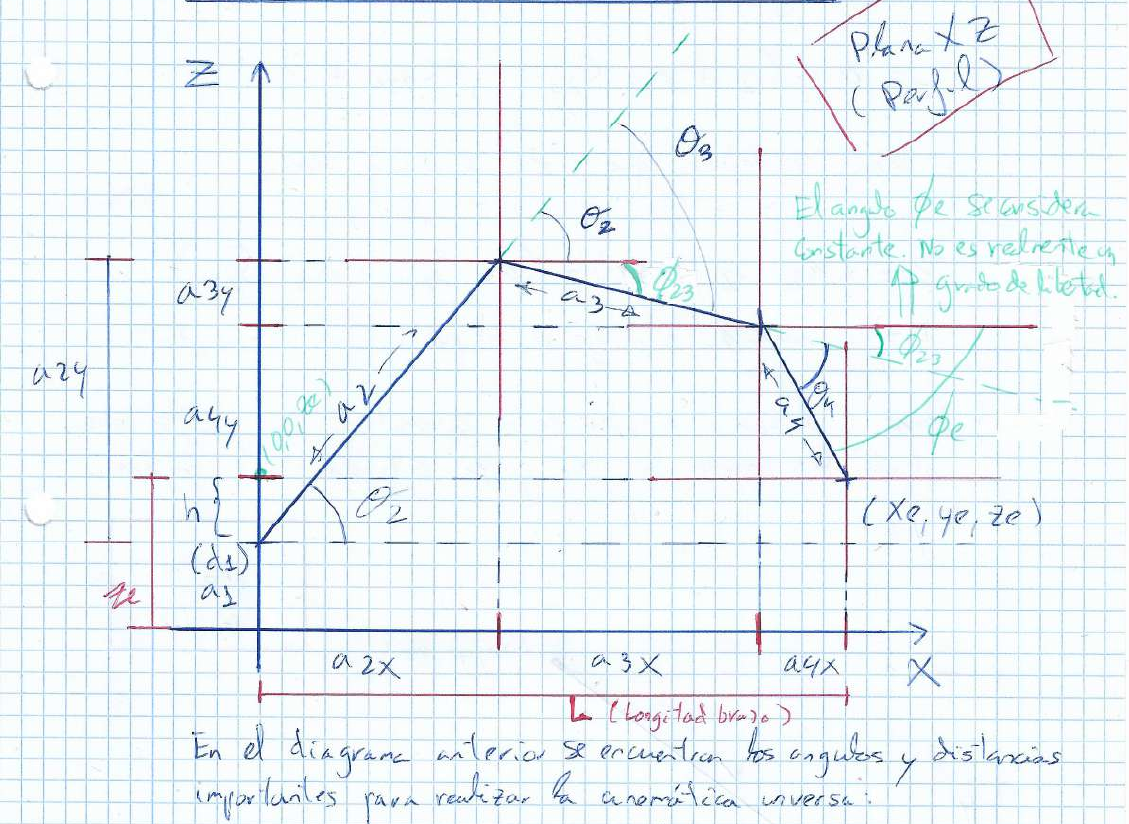
\includegraphics[width=.8\linewidth]{images/ik_geometry.png}
    \caption{distribución geométrica del brazo}
    \label{fig:ik_geometry}
\end{figure}

En la figura \ref{fig:ik_geometry} se puede ver cómo, en el plano $XZ$ (de perfil),
se encuentra presente una altura inicial $a_1$ correspondiente a la base del brazo,
así como una pequeña desviación en los ejes $d_1$ la cual afecta a la posición en $Z$.
A continuación, cada extremidad del brazo está definida junto con la correspondiente
articulación $\theta_i$. Como se puede observar, el ángulo $\theta_2$ es positivo pero,
debido a cómo está configurado el robot geométricamente, los ángulos $\theta_3$ y
$\theta_4$ han de ser negativos\footnote{véase la figura \ref{fig:sizes} para más
    información sobre la configuración del brazo robótico}.

Como se vio anteriormente en la sección \textit{Conocimientos previos},
en particular la figura \ref{fig:robot_config}, se suprimió el último parámetro de la
tabla de \textit{Denavit–Hartenberg} ya que dicho ángulo siempre es perpendicular al
plano del suelo y, por ende, está supeditado a los ángulos anteriores $\theta_2$ y
$\theta_3$. En su lugar, se sustituye por una traslación en el eje $Z$: $T_Z$ (véase
las matrices \ref{eq:A03_param} y \ref{eq:A03_num} y la ecuación \ref{eq:XeYeZe}).

De esta forma, se obtuvieron las siguientes ecuaciones para el plano $XZ$:

\begin{table}[H]
    \parbox{.45\linewidth}{
        \begin{equation} \label{eq:x_equations}
            L = \left\{\begin{aligned}
                a_{2X} & = a_2 \cdot \cos(\theta_2)            \\
                a_{3X} & = a_3 \cdot \cos(\theta_2 + \theta_3) \\
                a_{4X} & = a_4 \cdot \cos(\phi_e)              \\
            \end{aligned}
            \right.
        \end{equation}
    }
    \hfill
    \parbox{.45\linewidth}{
        \begin{equation} \label{eq:z_equations}
            H = \left\{\begin{aligned}
                a_{2Z} & = a_2 \cdot \sin(\theta_2)            \\
                a_{3Z} & = a_3 \cdot \sin(\theta_2 + \theta_3) \\
                a_{4Z} & = a_4 \cdot \sin(\phi_e)              \\
            \end{aligned}
            \right.
        \end{equation}
    }
\end{table}

Finalmente, se evaluó el plano $XY$ del modelo geométrico del brazo robótico:

\begin{figure}[H]
    \centering
    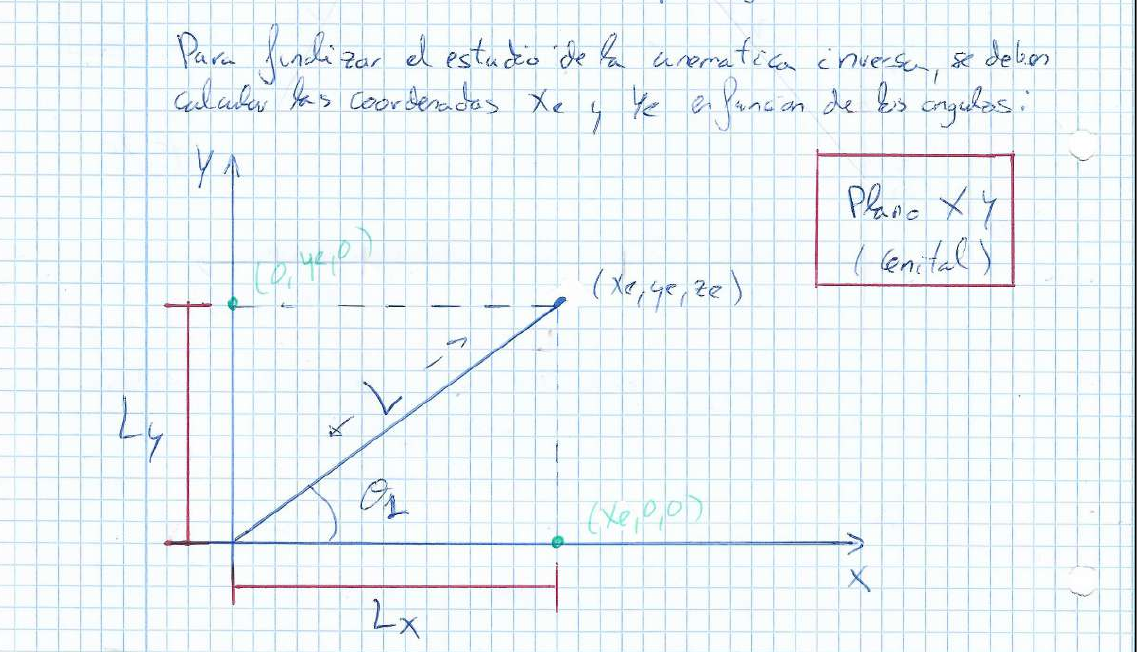
\includegraphics[width=.8\linewidth]{images/ik_xy_first_approach.png}
    \caption{plano $XY$ del brazo robótico}
    \label{fig:xy_first_approrach}
\end{figure}

De esta manera, se obtuvieron las siguientes ecuaciones para $L_X$ y $L_Y$:

\begin{equation} \label{eq:lx_ly_equations}
    \left\{
    \begin{aligned}
        L_X & = L \cdot \cos(\theta_1) = X_e \\
        L_Y & = L \cdot \sin(\theta_1) = Y_e \\
    \end{aligned}
    \right.
\end{equation}

La problemática de plantear el modelo de esta forma se mostró a la hora de intentar
resolver las ecuaciones de $X_e$, $Y_e$ y $Z_e$: al sustituir en la ecuación \ref{eq:XeYeZe},
el sistema a resolver era demasiado complejo, resultando imposible la obtención
de alguno de los ángulos, con lo que el sistema no tenía solución.

Como ya se comentó anteriormente, en la tabla de \textit{Denavit-Hartenberg} se eliminó
el último parámetro: pese a que sea un grado de libertad, al estar supeditado a los dos
ángulos anteriores y ser siempre perpendicular al plano del suelo, no es necesario
tenerlo en cuenta para la obtención de la inversa del robot.

Esto produjo que el último punto efectivo del robot resultara ser el extremo del brazo
de la articulación $\theta_3$:

\begin{figure}[H]
    \centering
    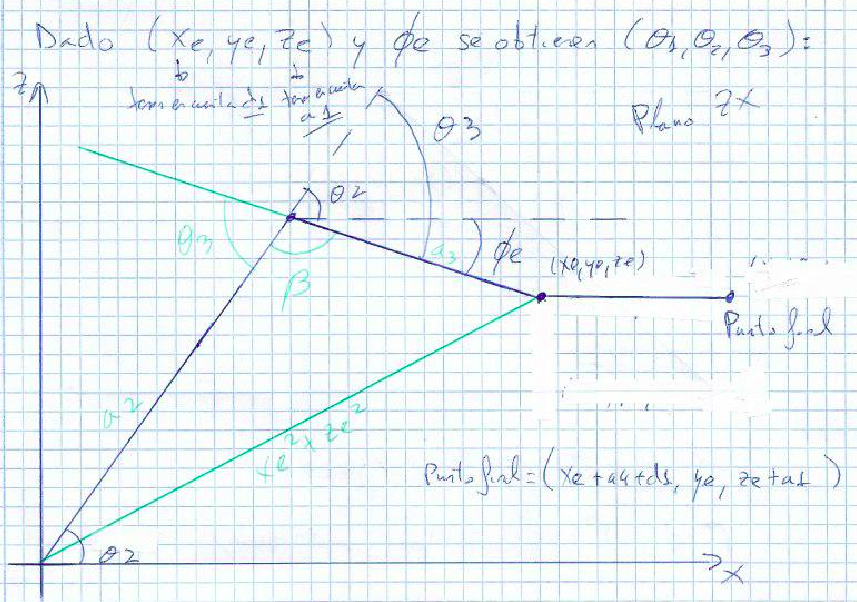
\includegraphics[width=.5\linewidth]{images/ik_schematic.png}
    \caption{aproximación geométrica del $\mu Arm$}
    \label{fig:ik_uarm}
\end{figure}

De esta forma, la complejidad se reduce bastante, ya que ahora en el plano $XZ$ solo
se cuentan con dos grados de libertad: $\theta_2$ y $\theta_3$, además de la traslación
en $X$ que se comentó anteriormente ($T_X$) y que se puede ver en la figura \ref{fig:ik_uarm}.

Esta nueva configuración permite aplicar el teorema del coseno\footnote
{Teorema del coseno: $c^2 = a^2 + b^2 - 2ab\cos\beta$}:

\begin{figure}[H]
    \centering
    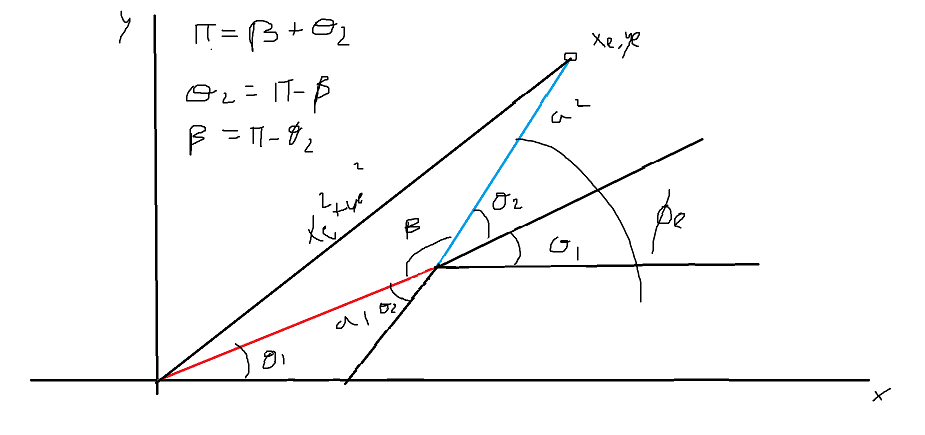
\includegraphics[width=.8\textwidth]{images/trigonometry.PNG}
    \caption{configuración del brazo robótico donde se puede aplicar el teorema del coseno}
    \label{fig:cos_theorem}
\end{figure}

Así, se pueden extraer $\theta_2$ y $\theta_3$:

\begin{align}
    \pi    & = \beta + \theta_3 \Longrightarrow \beta = \pi - \theta_3 \\
    \phi_e & = \theta_2 - \theta_3
\end{align}

Usando la ecuación \ref{eq:XeYeZe}, podemos despejar:

\begin{align*}
    X_e^2 + Z_e^2 & = a_2^2 + a_3^2 - 2a_2a_3\cos(\beta) =          \\
                  & = a_2^2 + a_3^2 - 2a_2a_3\cos(\pi - \theta_3) = \\
                  & = a_2^2 + a_3^2 + 2a_2a_3\cos(\theta_3)         \\
\end{align*}
\begin{align}
    \cos(\theta_3)           & = \frac{X_e^2 + Y_e^2 - a_2^2 - a_3^2}{2a_2a_3} \label{eq:cos_theta_3} \\
    \sin(\theta_3)           & = \sqrt{1 - \cos^2(\theta_3)} \label{eq:sin_theta_3}                   \\
    \Longrightarrow \theta_3 & = \arctan\left(\frac{\sin(\theta_3)}{\cos(\theta_3)}\right)
    \label{eq:theta_3}                                                                                \\
    \Longrightarrow \theta_2 & = \phi_e + \theta_3 \label{eq:theta_2}                                 \\
\end{align}

Finalmente, en el plano $XY$ tenemos la siguiente configuración:

\begin{figure}[H]
    \centering
    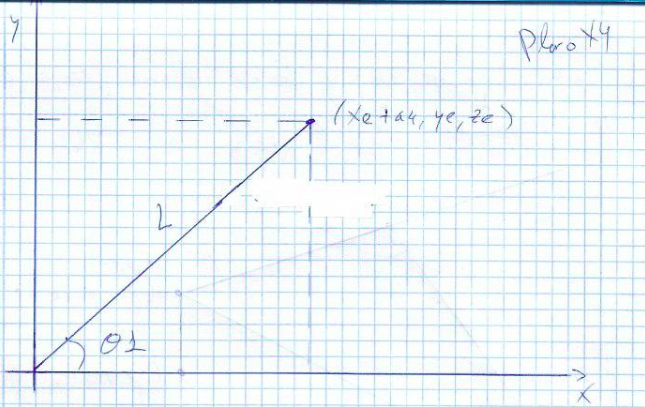
\includegraphics[width=.8\linewidth]{images/ik_xy_ok.png}
    \caption{visión del $\mu Arm$ en el plano $XY$}
    \label{fig:uarm_xy_ok}
\end{figure}

De este modo, aplicando el teorema de Pitágoras\footnote
{Teorema de Pitágoras: $h^2 = c_1^2 + c_2^2$}, se obtiene:

\begin{align*}
    L                              & = \pm \sqrt{(X_e + T_X)^2 + Y_e^2}                     \\
    \cos(\theta_1)                 & = \frac{X_e + T_X}{\sqrt{(X_e + T_X)^2 + Y_e^2 + d_1}} \\
    \sin(\theta_1)                 & = \frac{Y_e}{\sqrt{(X_e + T_X)^2 + Y_e + d_1}}         \\
    \Longrightarrow \tan(\theta_1) & = \frac{\sin(\theta_1)}{\cos(\theta_1)}                \\
\end{align*}
\begin{align}
    \theta_1 & = \arctan\left(\frac{\cfrac{Y_e}{\sqrt{(X_e + T_X)^2 + Y_e^2 + d_1}}}{\cfrac{X_e + T_X}{\sqrt{(X_e + T_X)^2 + Y_e^2 + d_1}}}\right) \\
             & = \arctan\left(\frac{Y_e}{X_e + T_X + d_1}\right) \label{eq:theta_1}                                                                \\
\end{align}

De esta forma, un algoritmo de obtención de la inversa sería:

\begin{itemize}
    \item Obtener $\theta_1$ a partir del punto $(X_e + T_X, Y_e, Z_e - T_Z)$, usando la ecuación \ref{eq:theta_1}.
    \item Obtener $(X_e ~ Y_e ~ Z_e)$ quitando las traslaciones $T_X$ y $T_Z$: $X_e = X_e - T_X; Z_e = Z_e + T_Z$.
    \item Obtener $\cos(\theta_3)$ con la ecuación \ref{eq:cos_theta_3} y el $\sin(\theta_3)$ con la ecuación \ref{eq:sin_theta_3}.
    \item Calcular $\theta_3$ usando la ecuación \ref{eq:theta_3}.
    \item Calcular $\theta_2$ usando la ecuación \ref{eq:theta_2}.
\end{itemize}

\section{Matriz Jacobiana}
\label{sec:jacobian}

La matriz Jacobiana nos permite obtener el movimiento $\vec{x}$, correspondiente a las
velocidades en el extremo del robot dadas unas velocidades de las articulaciones $\vec{q}$
\cite{travisdewolf_robot_2013}.

La matriz Jacobiana es una matriz de derivadas, esto es, varía según el tiempo. De esta forma,
se puede definir la matriz Jacobiana de un manipulador como:

\begin{equation} \label{eq:jacobian_manipulator}
    \vec{x} = J \cdot \vec{q}
    \left\{
    \begin{aligned}
        \vec{q} & = (\theta_1, \cdots, \theta_n, d_1, \cdots, d_n) \\
        \vec{x} & = (X_e, Y_e, Z_e, \phi_e)                        \\
        J       & \equiv matriz ~ Jacobiana
    \end{aligned}
    \right.
\end{equation}

\begin{align}
    J_1(\vec{q}) & =
    \begin{pmatrix}
        \frac{\partial X_e}{\partial q_0} & \frac{\partial X_e}{q_1} & \cdots & \frac{\partial X_e}{q_n} & \frac{\partial X_e}{d_1} & \cdots & \frac{\partial X_e}{d_n} \\
        \frac{\partial Y_e}{\partial q_0} & \frac{\partial Y_e}{q_1} & \cdots & \frac{\partial Y_e}{q_n} & \frac{\partial Y_e}{d_1} & \cdots & \frac{\partial Y_e}{d_n} \\
        \frac{\partial Z_e}{\partial q_0} & \frac{\partial Z_e}{q_1} & \cdots & \frac{\partial Z_e}{q_n} & \frac{\partial Z_e}{d_1} & \cdots & \frac{\partial Z_e}{d_n} \\
    \end{pmatrix} \label{eq:jacobian_1}
\end{align}
\begin{align}
    J_2(\vec{q}) & =
    \begin{pmatrix}
        \frac{\partial \phi_X}{\partial q_0} & \frac{\partial \phi_X}{q_1} & \cdots & \frac{\partial \phi_X}{q_n} & \frac{\partial \phi_X}{d_1} & \cdots & \frac{\partial \phi_X}{d_n} \\
        \frac{\partial \phi_Y}{\partial q_0} & \frac{\partial \phi_Y}{q_1} & \cdots & \frac{\partial \phi_Y}{q_n} & \frac{\partial \phi_Y}{d_1} & \cdots & \frac{\partial \phi_Y}{d_n} \\
        \frac{\partial \phi_Z}{\partial q_0} & \frac{\partial \phi_Z}{q_1} & \cdots & \frac{\partial \phi_Z}{q_n} & \frac{\partial \phi_Z}{d_1} & \cdots & \frac{\partial \phi_Z}{d_n} \\
    \end{pmatrix} \label{eq:jacobian_2}
\end{align}
\begin{align}
    J(\vec{q}) & =
    \begin{pmatrix}
        J_1(\vec{q}) \\
        J_2(\vec{q}) \\
    \end{pmatrix} \label{eq:jacobian}
\end{align}

En nuestro caso particular, obtenemos la siguiente matriz Jacobiana:

{\scriptsize\begin{align}
    J_1(\vec{q}) & =
    \begin{pmatrix}
        - \left(a_{2} \cos{\left(\theta_{2} \right)} + a_{3} \cos{\left(\theta_{2} - \theta_{3} \right)} + d_{1}\right) \sin{\left(\theta_{1} \right)} & \left(- a_{2} \sin{\left(\theta_{2} \right)} - a_{3} \sin{\left(\theta_{2} - \theta_{3} \right)}\right) \cos{\left(\theta_{1} \right)} & a_{3} \sin{\left(\theta_{2} - \theta_{3} \right)} \cos{\left(\theta_{1} \right)} \\
        \left(a_{2} \cos{\left(\theta_{2} \right)} + a_{3} \cos{\left(\theta_{2} - \theta_{3} \right)} + d_{1}\right) \cos{\left(\theta_{1} \right)}   & \left(- a_{2} \sin{\left(\theta_{2} \right)} - a_{3} \sin{\left(\theta_{2} - \theta_{3} \right)}\right) \sin{\left(\theta_{1} \right)} & a_{3} \sin{\left(\theta_{1} \right)} \sin{\left(\theta_{2} - \theta_{3} \right)} \\
        0                                                                                                                                              & a_{2} \cos{\left(\theta_{2} \right)} + a_{3} \cos{\left(\theta_{2} - \theta_{3} \right)}                                               & - a_{3} \cos{\left(\theta_{2} - \theta_{3} \right)}                              \\
    \end{pmatrix}
\end{align}}

\begin{align}
    J_2(\vec{q}) & =
    \begin{pmatrix}
        0 & 1 & -1 \\
        0 & 0 & 0  \\
        1 & 0 & 0  \\
    \end{pmatrix}
\end{align}

{\scriptsize\begin{align}
    J(\vec{q}) & =
    \begin{pmatrix}
        - \left(a_{2} \cos{\left(\theta_{2} \right)} + a_{3} \cos{\left(\theta_{2} - \theta_{3} \right)} + d_{1}\right) \sin{\left(\theta_{1} \right)} & \left(- a_{2} \sin{\left(\theta_{2} \right)} - a_{3} \sin{\left(\theta_{2} - \theta_{3} \right)}\right) \cos{\left(\theta_{1} \right)} & a_{3} \sin{\left(\theta_{2} - \theta_{3} \right)} \cos{\left(\theta_{1} \right)} \\
        \left(a_{2} \cos{\left(\theta_{2} \right)} + a_{3} \cos{\left(\theta_{2} - \theta_{3} \right)} + d_{1}\right) \cos{\left(\theta_{1} \right)}   & \left(- a_{2} \sin{\left(\theta_{2} \right)} - a_{3} \sin{\left(\theta_{2} - \theta_{3} \right)}\right) \sin{\left(\theta_{1} \right)} & a_{3} \sin{\left(\theta_{1} \right)} \sin{\left(\theta_{2} - \theta_{3} \right)} \\
        0                                                                                                                                              & a_{2} \cos{\left(\theta_{2} \right)} + a_{3} \cos{\left(\theta_{2} - \theta_{3} \right)}                                               & - a_{3} \cos{\left(\theta_{2} - \theta_{3} \right)}                              \\
        0                                                                                                                                              & 1                                                                                                                                      & -1                                                                               \\
        0                                                                                                                                              & 0                                                                                                                                      & 0                                                                                \\
        1                                                                                                                                              & 0                                                                                                                                      & 0                                                                                \\
    \end{pmatrix}
\end{align}}

Entre otras utilidades de la matriz Jacobiana, podemos obtener diferentes ecuaciones
que van relacionando el movimiento del brazo con el trabajo que hace, la fuerza que
es necesaria y la potencia:

\begin{align}
    W & = \int F^T \cdot v ~ dt              \\
    P & = \frac{W}{t} = \cdots = F^T \cdot v
\end{align}

Debido a la equivalencia energética, el trabajo se realiza a la misma velocidad,
independientemente del sistema \cite{travisdewolf_robot_2013}, por lo que se puede
escribir la potencia en términos del espacio del \textit{end-effector}:

\begin{align}
    P & = F_x^T \cdot \vec{x} \\
    P & = F_q^T \cdot \vec{q}
\end{align}

donde $F_x$ es la fuerza aplicada al brazo robótico y $\vec{x}$ la velocidad del mismo;
$F_q$ es el torque de las articulaciones y $\vec{q}$ es la velocidad angular de las mismas.

De esta información se deducen las matrices que conforman la Jacobiana. La ecuación
\ref{eq:jacobian_1} describe la velocidad lineal del \textit{end-effector}, y puede
ser escrita como $J_w(\vec{q})$; mientras, la ecuación \ref{eq:jacobian_2} describe la
velocidad angular del \textit{end-effector}, que puede ser escrita como $J_\omega(\vec{q})$.

Con la matriz Jacobiana ya obtenida se pueden obtener los puntos críticos. Dichos puntos
permiten conocer posiciones inalcanzables por el brazo robótico, ya que el determinante
en dicho punto es 0 y, por tanto, no existe la inversa.

Para este brazo robótico, el determinante es:

\begin{equation} \label{eq:det_j}
    |J(\vec{q})| = - a_{2} a_{3} \left(a_{2} \cos{\left(\theta_{2} \right)} + a_{3} \cos{\left(\theta_{2} - \theta_{3} \right)} + d_{1}\right) \sin{\left(\theta_{3} \right)}
\end{equation}

Analíticamente, los puntos críticos del $\mu Arm$ son: $\theta_3 = 0$ y $\theta_3 = \pi$.
Pero, al observar las tablas con los ángulos de giro de los motores (ver tabla \ref{tab:motors}),
comprobamos que el brazo robótico no es capaz de llegar a los $\ang{180}$ y, por la configuración
geométrica del mismo, tampoco puede tener $\ang{0}$\footnote
{el motor tiene esos grados de libertad, pero la articulación no, y está limitada por la estructura},
lo cual nos conduce a que no hay puntos críticos en este brazo robótico:

\begin{figure}[H]
    \centering
    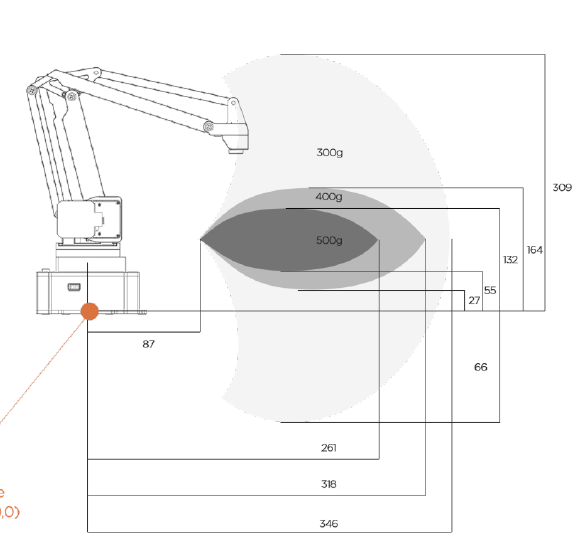
\includegraphics[width=.41\linewidth]{images/arm_weights_distances.png}
    \caption{área de trabajo del $\mu Arm$ \cite{noauthor_uarm_2019-1}}
    \label{fig:working_area}
\end{figure}

Igualmente, cuando se dan estos casos, se ha de hacer uso de o bien la matriz pseudo-inversa
($J^+$) de la matriz Jacobiana (si $J^{-1}$ no existe) o bien de la matriz transpuesta ($J^T$):

\begin{equation} \label{eq:pinv}
    J^+ = J^T \cdot \left(J \cdot J^T\right)^{-1}
\end{equation}

Una característica de la pseudo-inversa es que, en principio, siempre existe. Además,
si la inversa de la Jacobiana $J^{-1}$ existe, entonces la pseudo-inversa será igual a
la matriz inversa:

\begin{equation} \label{eq:pinv_exists}
    J^+ = J^{-1} \Leftrightarrow \exists ~ J^{-1}
\end{equation}

Esto se explica con mayor detalle en el punto \ref{sec:inv_jacobian}.

\subsection{Matriz Jacobiana inversa}
\label{sec:inv_jacobian}

La matriz Jacobiana inversa permite saber qué velocidad hay que aplicar en las
articulaciones $\vec{q}$ para obtener una velocidad en el \textit{end-effector}
$\vec{x}$.

En el caso del $\mu Arm$, la Jacobiana inversa resulta:

{\small\begin{align}
    J^{-1} & =
    \begin{pmatrix}
        - \frac{\sin{\left(\theta_{1} \right)}}{a_{2} \cos{\left(\theta_{2} \right)} + a_{3} \cos{\left(\theta_{2} - \theta_{3} \right)} + d_{1}}                                                 & \frac{\cos{\left(\theta_{1} \right)}}{a_{2} \cos{\left(\theta_{2} \right)} + a_{3} \cos{\left(\theta_{2} - \theta_{3} \right)} + d_{1}}                                                   & 0                                                                                                                                             \\
        - \frac{\cos{\left(\theta_{1} \right)} \cos{\left(\theta_{2} - \theta_{3} \right)}}{a_{2} \sin{\left(\theta_{3} \right)}}                                                                 & - \frac{\sin{\left(\theta_{1} \right)} \cos{\left(\theta_{2} - \theta_{3} \right)}}{a_{2} \sin{\left(\theta_{3} \right)}}                                                                 & - \frac{\sin{\left(\theta_{2} - \theta_{3} \right)}}{a_{2} \sin{\left(\theta_{3} \right)}}                                                    \\
        - \frac{\left(a_{2} \cos{\left(\theta_{2} \right)} + a_{3} \cos{\left(\theta_{2} - \theta_{3} \right)}\right) \cos{\left(\theta_{1} \right)}}{a_{2} a_{3} \sin{\left(\theta_{3} \right)}} & - \frac{\left(a_{2} \cos{\left(\theta_{2} \right)} + a_{3} \cos{\left(\theta_{2} - \theta_{3} \right)}\right) \sin{\left(\theta_{1} \right)}}{a_{2} a_{3} \sin{\left(\theta_{3} \right)}} & - \frac{a_{2} \sin{\left(\theta_{2} \right)} + a_{3} \sin{\left(\theta_{2} - \theta_{3} \right)}}{a_{2} a_{3} \sin{\left(\theta_{3} \right)}} \\
    \end{pmatrix}
\end{align}}

Como se observa en la ecuación \ref{eq:det_j}, el determinante del brazo robótico
se hace cero cuando el ángulo $\theta_3 = 0$ o bien cuando el mismo ángulo es $\pi$.
Pero, debido a la configuración geométrica del robot (ver figura \ref{fig:working_area}),
dichas configuraciones son inalcanzables.

Igualmente, para tratar configuraciones singulares, se utiliza la pseudo-inversa de
\textit{Moore-Penrose}. Dicha matriz existe y es única por cada matriz $A$ de entrada,
y se define según las ecuaciones \ref{eq:pinv} y \ref{eq:pinv_exists}.

Para el caso particular del $\mu Arm$, la pseudo-inversa es:

\begin{equation}
    J^+ =
    \begin{pmatrix}
        - \frac{\sin{\left(\theta_{1} \right)}}{a_{2} \cos{\left(\theta_{2} \right)} + a_{3} \cos{\left(\theta_{2} - \theta_{3} \right)} + d_{1}}                                                & \frac{\cos{\left(\theta_{1} \right)}}{a_{2}
        \cos{\left(\theta_{2} \right)} + a_{3} \cos{\left(\theta_{2} - \theta_{3} \right)} + d_{1}}                                                                                              & 0                                                                                                                                                                                                                                                                                                                                         \\
        - \frac{\cos{\left(\theta_{1} \right)} \cos{\left(\theta_{2} - \theta_{3} \right)}}{a_{2} \sin{\left(\theta_{3} \right)}}                                                                & - \frac{\sin{\left(\theta_{1} \right)} \cos{\left(\theta_{2} - \theta_{3} \right)}}{a_{2} \sin{\left(\theta_{3} \right)}}                                                                 & - \frac{\sin{\left(\theta_{2} - \theta_{3} \right)}}{a_{2} \sin{\left(\theta_{3} \right)}}                                                    \\
        - \frac{\left(a_{2} \cos{\left(\theta_{2} \right)} + a_{3} \cos{\left(\theta_{2} - \theta_{3} \right)}\right) \cos{\left(\theta_{1} \right)}}{a_{2} a_{3} \sin{\left(\theta_{3}\right)}} & - \frac{\left(a_{2} \cos{\left(\theta_{2} \right)} + a_{3} \cos{\left(\theta_{2} - \theta_{3} \right)}\right) \sin{\left(\theta_{1} \right)}}{a_{2} a_{3} \sin{\left(\theta_{3} \right)}} & - \frac{a_{2} \sin{\left(\theta_{2} \right)} + a_{3} \sin{\left(\theta_{2} - \theta_{3} \right)}}{a_{2} a_{3} \sin{\left(\theta_{3} \right)}}
    \end{pmatrix}
\end{equation}

Como se puede apreciar, la pseudo-inversa es exactamente igual que la inversa. Esto
es debido a que, como se muestra en la ecuación \ref{eq:pinv_exists}, la pseudo-inversa
es igual a la inversa siempre y cuando la inversa exista:

\begin{equation*}
    J^+ = J^{-1} \Leftrightarrow \exists ~ J^{-1}
\end{equation*}

Esto se cumple ya que es una de las propiedades de la inversa de \textit{Moore-Penrose}:

\begin{itemize}
    \item "\textit{if $A$ is invertible, its pseudo-inverse is its inverse. That is,
              $A^+ = A^{-1}$}" \cite{noauthor_moorepenrose_2019}.
\end{itemize}

\section{Planificación y descripción de una trayectoria}
\label{sec:trajectory}

Una trayectoria es el recorrido que debe describir un manipulador para cambiar su posición de un punto a otro.
La trayectoria que describe un manipulador está formada por un conjunto puntos cartesianos en el espacio,
es decir, puntos con tres coordenadas espaciales.

Para este caso, la trayectoria que va a describir el manipulador se define como:

\begin{equation}
    T = \left\{P_1, P_2, \cdots, P_{n}\right\} \backslash ~ P_k \in \field{R}^3, \forall k \in \left\{0, \cdots, n\right\}
\end{equation}

Un caso de interés a la hora de definir una trayectoria es en el que los puntos del recorrido
están definidos por una función matemática $f(x)$ de dos dimensiones. Dado que esta trayectoria
se define en un plano, una de las coordenadas se fija a cero. En el caso de usar $y = f_y(x)$,
el valor de la coordenada $z$ se fijaría a cero y por lo tanto la trayectoria estaría contenida
en el plano $XY$. De igual forma, en el caso de usar $z = f_z(x)$, el valor de la coordenada $y$
se fijaría a cero y por lo tanto la trayectoria estará contenida en el plano $XZ$.

En este caso y para simplificar la situación, la trayectoria se va describir en el plano $XY$,
siendo también posible aplicar este razonamiento para los planos $XZ$ o $YZ$. Para obtener
los puntos de la trayectoria, se debe muestrear la función $y = f_y(x)$ para ciertos valores de $x$
y, de esta forma, se obtendrían los puntos $P_{i} = \left(x, f_y(x), 0\right)$.

Dado que el $\mu Arm$ tiene una precisión mínima de movimiento de $0.2~mm.$ (en su \textit{end-effector}),
la función $f_y(x)$ se va a muestrear para valores de $x$ siguiendo la expresión
$x_{i} = x_{i-1} + 0,2 \cdot k$ con $k \in \field{N}$.
De esta manera, para cada valor de $x$ se obtiene un valor de $y$ y dado que $z$ es siempre nulo,
se obtienen todos los puntos de la trayectoria.

Una vez definida, el manipulador debe de moverse de un punto a otro siguiendo todos los puntos de la misma,
para así poder describir la función matemática. Para que esto ocurra, se debe determinar las coordenadas
articulares de los ejes de giro para todos y cada uno de los puntos y, de esta forma, se podrán controlar
los motores adecuadamente.

Para este manipulador, se han obtenido las expresiones explícitas de la cinemática inversa
(\textit{IK})\footnote{matrices de la cinemática inversa representadas en el punto 
\ref{sec:ik}, en particular las ecuaciones \ref{eq:theta_1}, \ref{eq:theta_2} y \ref{eq:theta_3}} y,
por lo tanto, para cada punto del espacio, se conoce exactamente las coordenadas articulares del mismo.
En el caso de no conocer las expresiones de la cinemática inversa, se podrían utilizar otros métodos de planificación
que aproximan la cinemática inversa, por ejemplo mediante el uso de la matriz Jacobiana.

En el gráfico siguiente se representa cómo, dados dos puntos en el espacio, se puede calcular
la variación de las coordenadas articulares necesaria para que el manipulador se desplace de un punto al otro:

\begin{figure}[H]
    \centering
    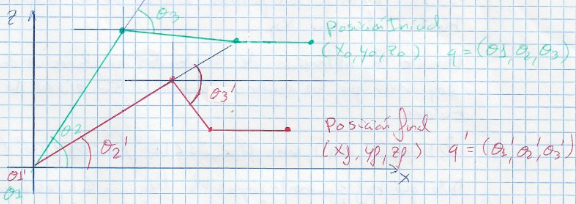
\includegraphics[width=.6\linewidth]{images/Trayectoria.png}
    \caption{descripción de la trayectoria del brazo robótico}
    \label{fig:trajectory}
\end{figure}

Dado el punto inicial ($P_o$) y punto final ($P_f$) de un desplazamiento, si se quiere calcular la variación que hay que aplicar
sobre las articulaciones para realizar dicho desplazamiento, se realizan los siguientes cálculos:
\begin{itemize}
    \item Se aplican las expresiones de cinemática inversa sobre el punto inicial $P_{o} = \left(x_{o}, y_{o}, z_{0}\right)$
          y punto final $P_{f} = \left(x_{f}, y_{f}, z_{f}\right)$ del desplazamiento, de forma que se obtienen las coordenadas
          articulares correspondientes a cada punto $q_{o} = \left({\theta_{1}}_o, {\theta_{2}}_o,{\theta_{3}}_o\right)$ y
          $q_{f} = \left({\theta_{1}}_f, {\theta_{2}}_f,{\theta_{3}}_f\right)$.
    \item Para calcular la variación en cada uno de los ángulos, se resta el vector de coordenadas articulares del punto final con las del punto inicial:
\end{itemize}
\begin{equation}
    \Delta q = \left({\theta_{1}}_f - {\theta_{1}}_o,{\theta_{2}}_f -{\theta_{2}}_o,{\theta_{3}}_f - {\theta_{3}}_o\right)
\end{equation}
\begin{itemize}
    \item Se aplica dicha variación de coordenadas articulares $\Delta q$ sobre los motores del manipulador para realizar el desplazamiento.
\end{itemize}

Una vez se ha descrito el proceso anterior, basta con aplicarlo de forma secuencial sobre todos los puntos de la
trayectoria calculados a partir de la función $f_y(x)$, desde el punto inicial $x_{1}$ de la trayectoria hasta el
punto final $x_{n}$; se consigue pues que las coordenadas articulares vayan variando progresivamente en cada uno
de los puntos de la trayectoria y por lo tanto el manipulador se desplaza.

Durante este proceso, se debe comprobar el valor de los ángulos de las coordenadas articulares para que estos no
excedan los límites reales de giro de cada una de las articulaciones. Además, dado que este manipulador tiene
posiciones singulares, pero no puede alcanzarlas debido al diseño físico, no existe problema al describir la trayectoria.

\newpage
\printbibliography

\end{document}